\documentclass[frenchb, paper=a4, fontsize=11pt]{scrartcl}

\usepackage[utf8x]{inputenc}
\usepackage[T1]{fontenc}
\usepackage{lmodern}

\usepackage{ifthen}
\usepackage{url}


\usepackage{multirow}

% Color
% cfr http://en.wikibooks.org/wiki/LaTeX/Colors
\usepackage{color}
\usepackage[usenames,dvipsnames,svgnames,table]{xcolor}
\definecolor{dkgreen}{rgb}{0.25,0.7,0.35}
\definecolor{dkred}{rgb}{0.7,0,0}

\newcommand{\matlab}{\textsc{Matlab}}

% Math symbols
\usepackage{amsmath}
\usepackage{amssymb}
\usepackage{amsthm}
\DeclareMathOperator*{\argmin}{arg\,min}
\DeclareMathOperator*{\argmax}{arg\,max}


% Sets
\newcommand{\Z}{\mathbb{Z}}
\newcommand{\R}{\mathbb{R}}
\newcommand{\Rn}{\R^n}
\newcommand{\Rnn}{\R^{n \times n}}
\newcommand{\C}{\mathbb{C}}
\newcommand{\K}{\mathbb{K}}
\newcommand{\Kn}{\K^n}
\newcommand{\Knn}{\K^{n \times n}}

% Unit vectors
\usepackage{esint}
\usepackage{esvect}
\newcommand{\kmath}{k}
\newcommand{\xunit}{\hat{\imath}}
\newcommand{\yunit}{\hat{\jmath}}
\newcommand{\zunit}{\hat{\kmath}}
\newcommand{\uunit}{\hat{\umath}}

% rot & div & grad & lap
\DeclareMathOperator{\newdiv}{div}
\newcommand{\divn}[1]{\nabla \cdot #1}
\newcommand{\rotn}[1]{\nabla \times #1}
\newcommand{\grad}[1]{\nabla #1}
\newcommand{\gradn}[1]{\nabla #1}
\newcommand{\lap}[1]{\nabla^2 #1}


% Elec
\newcommand{\B}{\vec B}
\newcommand{\E}{\vec E}
\newcommand{\EMF}{\mathcal{E}}
\newcommand{\perm}{\varepsilon} % permittivity

\newcommand{\bigoh}{\mathcal{O}}
\newcommand\eqdef{\triangleq}

\DeclareMathOperator{\newdiff}{d} % use \dif instead
\newcommand{\dif}{\newdiff\!}
\newcommand{\fpart}[2]{\frac{\partial #1}{\partial #2}}
\newcommand{\ffpart}[2]{\frac{\partial^2 #1}{\partial #2^2}}
\newcommand{\fdpart}[3]{\frac{\partial^2 #1}{\partial #2\partial #3}}
\newcommand{\fdif}[2]{\frac{\dif #1}{\dif #2}}
\newcommand{\ffdif}[2]{\frac{\dif^2 #1}{\dif #2^2}}
\newcommand{\constant}{\ensuremath{\mathrm{cst}}}

\usepackage{siunitx}

\usepackage{tikz}
\usepackage{tikz-3dplot}

\usepackage{pgfplots}
\usepackage{lmodern}
%\usepackage[protrusion=true,expansion=true]{microtype}
\usepackage{xspace}

\usepackage{babel}
% Listing
% always put it after babel
% http://tex.stackexchange.com/questions/100717/code-in-lstlisting-breaks-document-compile-error
\usepackage{listings}

\definecolor{mygreen}{rgb}{0,0.6,0}
\definecolor{mygray}{rgb}{0.5,0.5,0.5}
\definecolor{mymauve}{rgb}{0.58,0,0.82}
\lstset{ %
  language=Matlab,
  backgroundcolor=\color{white},   % choose the background color; you must add \usepackage{color} or \usepackage{xcolor}
  basicstyle=\footnotesize,        % the size of the fonts that are used for the code
  breakatwhitespace=false,         % sets if automatic breaks should only happen at whitespace
  breaklines=true,                 % sets automatic line breaking
  captionpos=b,                    % sets the caption-position to bottom
  commentstyle=\color{mygreen},    % comment style
  deletekeywords={...},            % if you want to delete keywords from the given language
  escapeinside={\%*}{*)},          % if you want to add LaTeX within your code
  extendedchars=true,              % lets you use non-ASCII characters; for 8-bits encodings only, does not work with UTF-8
  frame=single,	                   % adds a frame around the code
  keepspaces=true,                 % keeps spaces in text, useful for keeping indentation of code (possibly needs columns=flexible)
  keywordstyle=\color{blue},       % keyword style
  otherkeywords={*,...},           % if you want to add more keywords to the set
  numbers=none,                    % where to put the line-numbers; possible values are (none, left, right)
  numbersep=5pt,                   % how far the line-numbers are from the code
  numberstyle=\tiny\color{mygray}, % the style that is used for the line-numbers
  rulecolor=\color{black},         % if not set, the frame-color may be changed on line-breaks within not-black text (e.g. comments (green here))
  showspaces=false,                % show spaces everywhere adding particular underscores; it overrides 'showstringspaces'
  showstringspaces=false,          % underline spaces within strings only
  showtabs=false,                  % show tabs within strings adding particular underscores
  stepnumber=2,                    % the step between two line-numbers. If it's 1, each line will be numbered
  stringstyle=\color{mymauve},     % string literal style
  tabsize=2,	                   % sets default tabsize to 2 spaces
  title=\lstname                   % show the filename of files included with \lstinputlisting; also try caption instead of title
}

\KOMAoptions{DIV=last}

\usepackage[top = 2.5 cm, bottom = 3 cm, left = 2.5 cm, right = 2.5 cm]{geometry}
\usepackage{hyperref}
\usepackage{todonotes}
\DeclareSIUnit{\rot}{rot}
\usepackage[makeroom]{cancel}

%%% Custom sectioning (sectsty package)
\usepackage{sectsty}								% Custom sectioning (see below)
\allsectionsfont{\scshape}						% Change font of al section commands

%%% Custom headers/footers (fancyhdr package)
\usepackage{fancyhdr}
\pagestyle{fancyplain}
\fancyhead{}										% No page header
\fancyfoot[L]{\small Groupe 1}					% You may remove/edit this line 
\fancyfoot[C]{}									% Empty
\fancyfoot[R]{\thepage}							% Pagenumbering
\renewcommand{\headrulewidth}{0pt}				% Remove header underlines
\renewcommand{\footrulewidth}{0pt}				% Remove footer underlines
\setlength{\headheight}{13.6pt}

%%% Equation and float numbering
\numberwithin{equation}{section}					% Equationnumbering: section.eq#
\numberwithin{figure}{section}					% Figurenumbering: section.fig#
\numberwithin{table}{section}						% Tablenumbering: section.tab#

%%% Maketitle metadata
\newcommand{\horrule}[1]{\rule{\linewidth}{#1}} 	% Horizontal rule

\title{
		%\vspace{-1in} 	
		\usefont{OT1}{bch}{b}{n}
		\normalfont \normalsize \textsc{Ecole polytechnique de Louvain} \\ [25pt]
		\horrule{0.5pt} \\[0.4cm]
		\large LINMA1510 - Automatique linéaire\\
		\huge Laboratoire 2 - Contrôle d'un moteur à courant continu \\
		\horrule{1.5pt} \\[0.5cm]
}
\author{
		\normalfont
		\textsc{Groupe 62}\\
      	Antoine Paris\hspace{0.6cm} Philippe Verbist \\	
       	\normalsize
        \today
}
\date{}

\begin{document}
\maketitle

\section{Identification du modèle}
En boucle ouverte, la fonction de transfert du moteur à courant
continu est celle d'un système du premier ordre
\begin{equation}
	G(s) = \frac{K}{1+s\tau}
\end{equation}
où $K$ est le gain statique et $\tau$ la constante de temps.
On applique ensuite un échelon d'amplitude \SI{6}{\volt} en
entrée (on passe de \SI{3}{\volt} à \SI{9}{\volt}). La
transformée de Laplace d'un échelon d'amplitude $a$ est donnée
par
\begin{equation}
	\frac{a}{s}
\end{equation}
et donc la sortie $Y(s)$ est donnée par
\begin{equation}
	Y(s) = \frac{K}{1+s\tau}\cdot\frac{a}{s}.
\end{equation}
Dans le domaine temporel, on a alors pour $t > 0$
\begin{equation}
	y(t) = K(1-e^{-\frac{t}{\tau}})a.
\end{equation}
Le résultat de la mesure sur le moteur DC est donné à la figure
\ref{fig:open-loop-step-response}. En isolant la partie régime
permanent et en prenant la moyenne de la vitesse angulaire sur
cette partie, on trouve que
\begin{equation}
	\lim_{t\to\infty} y(t) = \SI{16.15}{\rot\per\second}.
\end{equation}
Comme ici l'amplitude de l'échelon est de \SI{6}{\volt} et qu'on
démarre de \SI{3}{\volt}, on obtient
\begin{equation}
	K = \frac{16.15-3}{6} = \SI{2.1917}{\rot\per\second\per\volt}.
\end{equation}
On trouve également de manière expérimentale par essai/erreur en
s'arrangeant pour que la courbe théorique colle le mieux possible
à la courbe expérimentale
\begin{equation}
	\tau = \SI{0.8}{\second}.
\end{equation}
Le modèle obtenu est confronté aux mesures expérimentales à la
figure \ref{fig:open-loop-step-response_model}. On constate que
le modèle colle assez bien à la réalité.

\begin{figure}[ht]
	\centering
	% This file was created by matlab2tikz.
%
%The latest updates can be retrieved from
%  http://www.mathworks.com/matlabcentral/fileexchange/22022-matlab2tikz-matlab2tikz
%where you can also make suggestions and rate matlab2tikz.
%
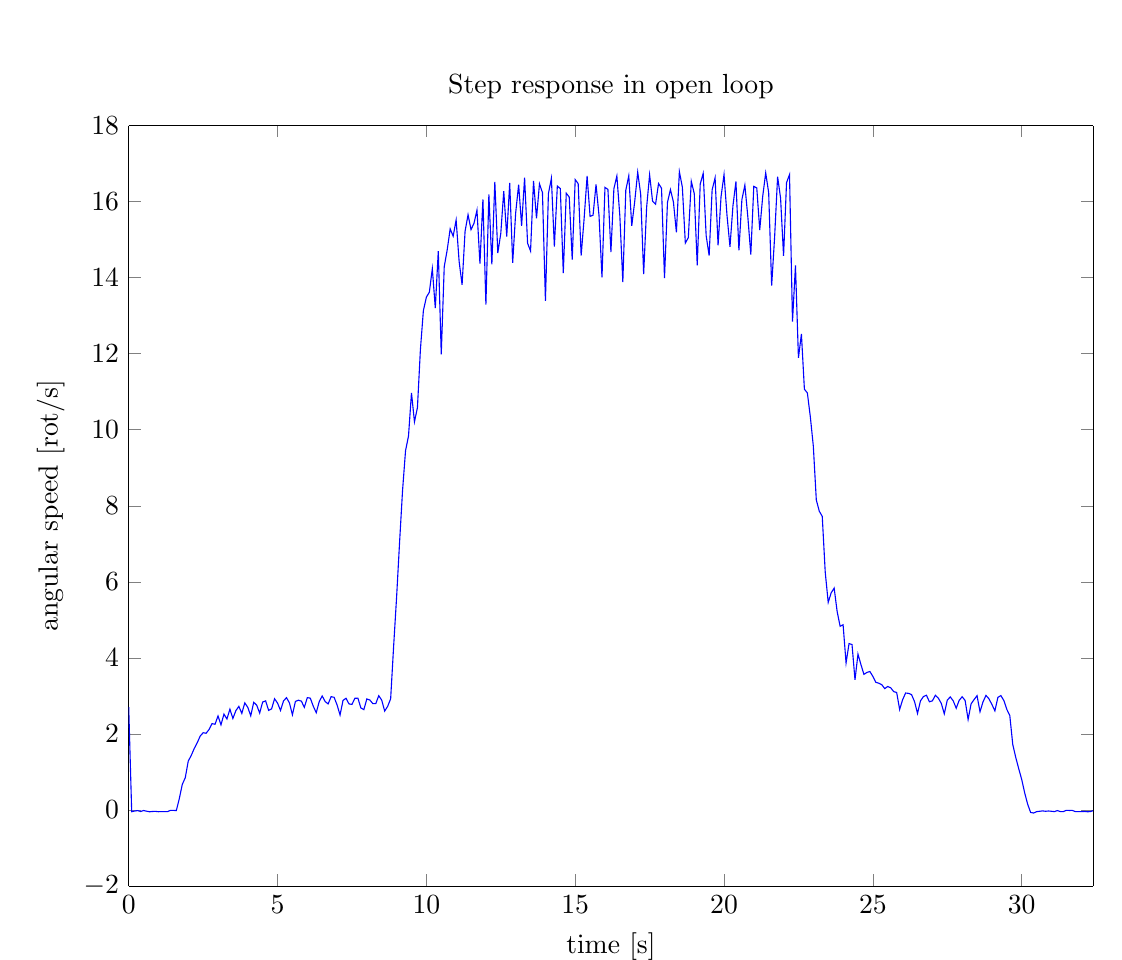
\begin{tikzpicture}

\begin{axis}[%
width=4.822in,
height=3.803in,
at={(0.809in,0.513in)},
scale only axis,
separate axis lines,
every outer x axis line/.append style={black},
every x tick label/.append style={font=\color{black}},
xmin=0,
xmax=32.4,
xlabel={time [s]},
every outer y axis line/.append style={black},
every y tick label/.append style={font=\color{black}},
ymin=-2,
ymax=18,
ylabel={angular speed [rot/s]},
axis background/.style={fill=white},
title={Step response in open loop}
]
\addplot [color=blue,solid,forget plot]
  table[row sep=crcr]{%
0	2.706113\\
0.1	-0.042591357\\
0.2	-0.026116869\\
0.3	-0.013444186\\
0.4	-0.038789552\\
0.5	-0.012176917\\
0.6	-0.029918674\\
0.7	-0.045125894\\
0.8	-0.037522284\\
0.9	-0.034987747\\
1	-0.043858626\\
1.1	-0.040056821\\
1.2	-0.041324089\\
1.3	-0.042591357\\
1.4	-0.008375112\\
1.5	-0.009642381\\
1.6	-0.012176917\\
1.7	0.30210562\\
1.8	0.674682482\\
1.9	0.849565492\\
2	1.286773\\
2.1	1.435043\\
2.2	1.616263\\
2.3	1.7658\\
2.4	1.943218\\
2.5	2.033194\\
2.6	2.019254\\
2.7	2.119368\\
2.8	2.272708\\
2.9	2.256233\\
3	2.472936\\
3.1	2.241026\\
3.2	2.522359\\
3.3	2.394365\\
3.4	2.652888\\
3.5	2.408305\\
3.6	2.613603\\
3.7	2.726389\\
3.8	2.541368\\
3.9	2.8189\\
4	2.701044\\
4.1	2.478005\\
4.2	2.834107\\
4.3	2.756804\\
4.4	2.551506\\
4.5	2.840444\\
4.6	2.870858\\
4.7	2.621206\\
4.8	2.659224\\
4.9	2.926618\\
5	2.812564\\
5.1	2.618672\\
5.2	2.868323\\
5.3	2.955765\\
5.4	2.816365\\
5.5	2.505885\\
5.6	2.855651\\
5.7	2.8886\\
5.8	2.864522\\
5.9	2.701044\\
6	2.955765\\
6.1	2.943092\\
6.2	2.731458\\
6.3	2.55911\\
6.4	2.849314\\
6.5	3.000119\\
6.6	2.853116\\
6.7	2.79102\\
6.8	2.98111\\
6.9	2.964636\\
7	2.764407\\
7.1	2.499548\\
7.2	2.882263\\
7.3	2.93929\\
7.4	2.79102\\
7.5	2.778347\\
7.6	2.93929\\
7.7	2.941825\\
7.8	2.683302\\
7.9	2.641482\\
8	2.921549\\
8.1	2.893669\\
8.2	2.799891\\
8.3	2.797356\\
8.4	3.006456\\
8.5	2.8886\\
8.6	2.602197\\
8.7	2.727657\\
8.8	2.924083\\
8.9	4.305405\\
9	5.600552\\
9.1	7.042703\\
9.2	8.403748\\
9.3	9.447976\\
9.4	9.837027\\
9.5	10.971231\\
9.6	10.208336\\
9.7	10.58218\\
9.8	12.113038\\
9.9	13.134455\\
10	13.485488\\
10.1	13.617284\\
10.2	14.23571\\
10.3	13.199086\\
10.4	14.698262\\
10.5	11.983777\\
10.6	14.286401\\
10.7	14.731211\\
10.8	15.282472\\
10.9	15.088581\\
11	15.515649\\
11.1	14.429602\\
11.2	13.808641\\
11.3	15.216575\\
11.4	15.653782\\
11.5	15.262196\\
11.6	15.428208\\
11.7	15.774172\\
11.8	14.368773\\
11.9	16.056772\\
12	13.287795\\
12.1	16.188568\\
12.2	14.351031\\
12.3	16.515523\\
12.4	14.647572\\
12.5	15.162082\\
12.6	16.274742\\
12.7	15.082244\\
12.8	16.487643\\
12.9	14.391584\\
13	15.701938\\
13.1	16.444556\\
13.2	15.364845\\
13.3	16.630844\\
13.4	14.906094\\
13.5	14.69953\\
13.6	16.54467\\
13.7	15.557469\\
13.8	16.468634\\
13.9	16.235457\\
14	13.39171\\
14.1	16.208844\\
14.2	16.610568\\
14.3	14.817386\\
14.4	16.407805\\
14.5	16.341907\\
14.6	14.116587\\
14.7	16.218983\\
14.8	16.117601\\
14.9	14.475224\\
15	16.576352\\
15.1	16.472436\\
15.2	14.581674\\
15.3	15.554935\\
15.4	16.671397\\
15.5	15.609427\\
15.6	15.642376\\
15.7	16.449625\\
15.8	15.634773\\
15.9	14.006335\\
16	16.372322\\
16.1	16.319097\\
16.2	14.674184\\
16.3	16.338106\\
16.4	16.672664\\
16.5	15.6221\\
16.6	13.884677\\
16.7	16.29882\\
16.8	16.676466\\
16.9	15.359776\\
17	16.004814\\
17.1	16.774045\\
17.2	16.19237\\
17.3	14.091242\\
17.4	15.85401\\
17.5	16.703078\\
17.6	16.007349\\
17.7	15.928778\\
17.8	16.473703\\
17.9	16.352046\\
18	13.987326\\
18.1	15.980736\\
18.2	16.314028\\
18.3	15.98834\\
18.4	15.188695\\
18.5	16.785451\\
18.6	16.378658\\
18.7	14.909896\\
18.8	15.050563\\
18.9	16.534532\\
19	16.208844\\
19.1	14.324419\\
19.2	16.459763\\
19.3	16.742364\\
19.4	15.102521\\
19.5	14.579139\\
19.6	16.305157\\
19.7	16.623241\\
19.8	14.8478\\
19.9	16.129007\\
20	16.710682\\
20.1	15.637307\\
20.2	14.812316\\
20.3	15.889493\\
20.4	16.526928\\
20.5	14.716004\\
20.6	16.049169\\
20.7	16.431883\\
20.8	15.596755\\
20.9	14.605752\\
21	16.400202\\
21.1	16.358382\\
21.2	15.253325\\
21.3	16.137877\\
21.4	16.753769\\
21.5	16.23419\\
21.6	13.788365\\
21.7	15.072106\\
21.8	16.654922\\
21.9	16.089721\\
22	14.571536\\
22.1	16.496514\\
22.2	16.708147\\
22.3	12.841717\\
22.4	14.31935\\
22.5	11.888732\\
22.6	12.519831\\
22.7	11.066276\\
22.8	10.967429\\
22.9	10.33633\\
23	9.569633\\
23.1	8.155363\\
23.2	7.858823\\
23.3	7.721958\\
23.4	6.254462\\
23.5	5.461153\\
23.6	5.712072\\
23.7	5.836264\\
23.8	5.220372\\
23.9	4.833856\\
24	4.873141\\
24.1	3.86693\\
24.2	4.378907\\
24.3	4.351027\\
24.4	3.424654\\
24.5	4.101375\\
24.6	3.823843\\
24.7	3.567855\\
24.8	3.618546\\
24.9	3.643891\\
25	3.51463\\
25.1	3.358756\\
25.2	3.335945\\
25.3	3.29666\\
25.4	3.192744\\
25.5	3.249771\\
25.6	3.214288\\
25.7	3.114173\\
25.8	3.091363\\
25.9	2.645284\\
26	2.901272\\
26.1	3.077423\\
26.2	3.068552\\
26.3	3.035603\\
26.4	2.851849\\
26.5	2.540101\\
26.6	2.870858\\
26.7	2.984912\\
26.8	3.019128\\
26.9	2.84678\\
27	2.870858\\
27.1	3.017861\\
27.2	2.943092\\
27.3	2.802426\\
27.4	2.53123\\
27.5	2.8886\\
27.6	2.976041\\
27.7	2.872125\\
27.8	2.676966\\
27.9	2.884798\\
28	2.979843\\
28.1	2.880996\\
28.2	2.381693\\
28.3	2.79102\\
28.4	2.905074\\
28.5	3.007723\\
28.6	2.584455\\
28.7	2.842978\\
28.8	3.014059\\
28.9	2.92535\\
29	2.775813\\
29.1	2.608534\\
29.2	2.962101\\
29.3	3.010257\\
29.4	2.880996\\
29.5	2.647819\\
29.6	2.48941\\
29.7	1.725248\\
29.8	1.386887\\
29.9	1.087812\\
30	0.806478374\\
30.1	0.454177811\\
30.2	0.1551025\\
30.3	-0.062867651\\
30.4	-0.078074871\\
30.5	-0.042591357\\
30.6	-0.032453211\\
30.7	-0.022315064\\
30.8	-0.032453211\\
30.9	-0.024849601\\
31	-0.032453211\\
31.1	-0.041324089\\
31.2	-0.013444186\\
31.3	-0.041324089\\
31.4	-0.040056821\\
31.5	-0.007107844\\
31.6	-0.010909649\\
31.7	-0.009642381\\
31.8	-0.040056821\\
31.9	-0.042591357\\
32	-0.040056821\\
32.1	-0.036255016\\
32.2	-0.043858626\\
32.3	-0.042591357\\
32.4	-0.015978722\\
};
\end{axis}
\end{tikzpicture}%
	\caption{Réponse indicielle en boucle ouverte.}
	\label{fig:open-loop-step-response}
\end{figure}

\begin{figure}[ht]
	\centering
	% This file was created by matlab2tikz.
%
%The latest updates can be retrieved from
%  http://www.mathworks.com/matlabcentral/fileexchange/22022-matlab2tikz-matlab2tikz
%where you can also make suggestions and rate matlab2tikz.
%
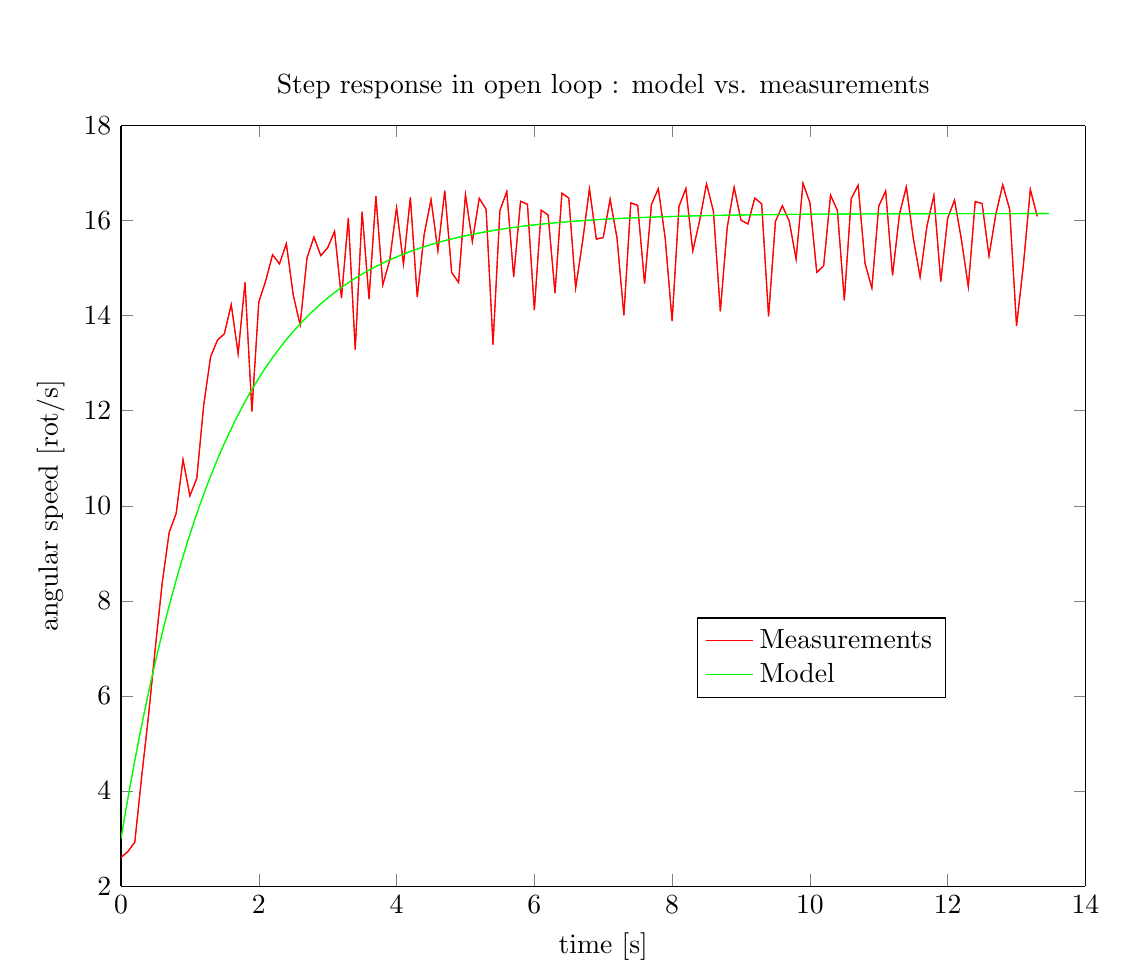
\begin{tikzpicture}

\begin{axis}[%
width=4.822in,
height=3.803in,
at={(0.809in,0.513in)},
scale only axis,
separate axis lines,
every outer x axis line/.append style={black},
every x tick label/.append style={font=\color{black}},
xmin=0,
xmax=14,
xlabel={time [s]},
every outer y axis line/.append style={black},
every y tick label/.append style={font=\color{black}},
ymin=2,
ymax=18,
ylabel={angular speed [rot/s]},
axis background/.style={fill=white},
title={Step response in open loop : model vs. measurements},
legend style={at={(0.597,0.247)},anchor=south west,legend cell align=left,align=left,draw=black}
]
\addplot [color=red,solid]
  table[row sep=crcr]{%
0	2.602197\\
0.0999999999999996	2.727657\\
0.200000000000001	2.924083\\
0.300000000000001	4.305405\\
0.4	5.600552\\
0.5	7.042703\\
0.6	8.403748\\
0.700000000000001	9.447976\\
0.800000000000001	9.837027\\
0.9	10.971231\\
1	10.208336\\
1.1	10.58218\\
1.2	12.113038\\
1.3	13.134455\\
1.4	13.485488\\
1.5	13.617284\\
1.6	14.23571\\
1.7	13.199086\\
1.8	14.698262\\
1.9	11.983777\\
2	14.286401\\
2.1	14.731211\\
2.2	15.282472\\
2.3	15.088581\\
2.4	15.515649\\
2.5	14.429602\\
2.6	13.808641\\
2.7	15.216575\\
2.8	15.653782\\
2.9	15.262196\\
3	15.428208\\
3.1	15.774172\\
3.2	14.368773\\
3.3	16.056772\\
3.4	13.287795\\
3.5	16.188568\\
3.6	14.351031\\
3.7	16.515523\\
3.8	14.647572\\
3.9	15.162082\\
4	16.274742\\
4.1	15.082244\\
4.2	16.487643\\
4.3	14.391584\\
4.4	15.701938\\
4.5	16.444556\\
4.6	15.364845\\
4.7	16.630844\\
4.8	14.906094\\
4.9	14.69953\\
5	16.54467\\
5.1	15.557469\\
5.2	16.468634\\
5.3	16.235457\\
5.4	13.39171\\
5.5	16.208844\\
5.6	16.610568\\
5.7	14.817386\\
5.8	16.407805\\
5.9	16.341907\\
6	14.116587\\
6.1	16.218983\\
6.2	16.117601\\
6.3	14.475224\\
6.4	16.576352\\
6.5	16.472436\\
6.6	14.581674\\
6.7	15.554935\\
6.8	16.671397\\
6.9	15.609427\\
7	15.642376\\
7.1	16.449625\\
7.2	15.634773\\
7.3	14.006335\\
7.4	16.372322\\
7.5	16.319097\\
7.6	14.674184\\
7.7	16.338106\\
7.8	16.672664\\
7.9	15.6221\\
8	13.884677\\
8.1	16.29882\\
8.2	16.676466\\
8.3	15.359776\\
8.4	16.004814\\
8.5	16.774045\\
8.6	16.19237\\
8.7	14.091242\\
8.8	15.85401\\
8.9	16.703078\\
9	16.007349\\
9.1	15.928778\\
9.2	16.473703\\
9.3	16.352046\\
9.4	13.987326\\
9.5	15.980736\\
9.6	16.314028\\
9.7	15.98834\\
9.8	15.188695\\
9.9	16.785451\\
10	16.378658\\
10.1	14.909896\\
10.2	15.050563\\
10.3	16.534532\\
10.4	16.208844\\
10.5	14.324419\\
10.6	16.459763\\
10.7	16.742364\\
10.8	15.102521\\
10.9	14.579139\\
11	16.305157\\
11.1	16.623241\\
11.2	14.8478\\
11.3	16.129007\\
11.4	16.710682\\
11.5	15.637307\\
11.6	14.812316\\
11.7	15.889493\\
11.8	16.526928\\
11.9	14.716004\\
12	16.049169\\
12.1	16.431883\\
12.2	15.596755\\
12.3	14.605752\\
12.4	16.400202\\
12.5	16.358382\\
12.6	15.253325\\
12.7	16.137877\\
12.8	16.753769\\
12.9	16.23419\\
13	13.788365\\
13.1	15.072106\\
13.2	16.654922\\
13.3	16.089721\\
};
\addlegendentry{Measurements};

\addplot [color=green,solid]
  table[row sep=crcr]{%
0	3\\
0.0690775527897984	3.59184749381792\\
0.138155105579597	4.15705746246942\\
0.207232658369395	4.69682879207701\\
0.276310211159194	5.21230640999921\\
0.345387763948992	5.7045837133749\\
0.41446531673879	6.17470488836532\\
0.483542869528589	6.62366712501286\\
0.552620422318387	7.05242273241487\\
0.621697975108185	7.46188115869891\\
0.690775527897984	7.85291092008419\\
0.759853080687782	8.22634144312086\\
0.828930633477581	8.58296482401499\\
0.898008186267379	8.9235375087708\\
0.967085739057177	9.24878189771401\\
1.03616329184698	9.55938787779985\\
1.10524084463677	9.85601428595576\\
1.17431839742657	10.1392903065628\\
1.24339595021637	10.4098168060402\\
1.31247350300617	10.6681676073635\\
1.38155105579597	10.9148907072199\\
1.45062860858577	11.150509438383\\
1.51970616137556	11.3755235797716\\
1.58878371416536	11.5904104165476\\
1.65786126695516	11.7956257525023\\
1.72693881974496	11.991604876877\\
1.79601637253476	12.1787634876698\\
1.86509392532456	12.3574985733869\\
1.93417147811435	12.5281892551087\\
2.00324903090415	12.691197590656\\
2.07232658369395	12.8468693425634\\
2.14140413648375	12.9955347114879\\
2.21048168927355	13.1375090366089\\
2.27955924206335	13.2730934645049\\
2.34863679485315	13.4025755879255\\
2.41771434764294	13.5262300558145\\
2.48679190043274	13.6443191558769\\
2.55586945322254	13.7570933709265\\
2.62494700601234	13.8647919101932\\
2.69402455880214	13.9676432167183\\
2.76310211159194	14.0658654519123\\
2.83217966438173	14.1596669583051\\
2.90125721717153	14.2492467014679\\
2.97033476996133	14.334794692046\\
3.03941232275113	14.4164923887971\\
3.10848987554093	14.4945130834895\\
3.17756742833073	14.569022268477\\
3.24664498112052	14.6401779877305\\
3.31572253391032	14.7081311720706\\
3.38480008670012	14.773025959312\\
3.45387763948992	14.834999999999\\
3.52295519227972	14.8941847493808\\
3.59203274506952	14.950705746246\\
3.66111029785931	15.0046828792068\\
3.73018785064911	15.0562306409991\\
3.79926540343891	15.1054583713367\\
3.86834295622871	15.1524704888358\\
3.93742050901851	15.1973667125005\\
4.00649806180831	15.2402422732408\\
4.0755756145981	15.2811881158692\\
4.1446531673879	15.3202910920078\\
4.2137307201777	15.3576341443115\\
4.2828082729675	15.3932964824009\\
4.3518858257573	15.4273537508765\\
4.4209633785471	15.4598781897709\\
4.49004093133689	15.4909387877795\\
4.55911848412669	15.5206014285951\\
4.62819603691649	15.5489290306558\\
4.69727358970629	15.5759816806036\\
4.76635114249609	15.6018167607359\\
4.83542869528589	15.6264890707216\\
4.90450624807568	15.6500509438379\\
4.97358380086548	15.6725523579768\\
5.04266135365528	15.6940410416544\\
5.11173890644508	15.7145625752499\\
5.18081645923488	15.7341604876874\\
5.24989401202468	15.7528763487667\\
5.31897156481448	15.7707498573384\\
5.38804911760427	15.7878189255106\\
5.45712667039407	15.8041197590653\\
5.52620422318387	15.8196869342561\\
5.59528177597367	15.8345534711485\\
5.66435932876347	15.8487509036606\\
5.73343688155327	15.8623093464502\\
5.80251443434306	15.8752575587923\\
5.87159198713286	15.8876230055812\\
5.94066953992266	15.8994319155875\\
6.00974709271246	15.9107093370925\\
6.07882464550226	15.9214791910191\\
6.14790219829206	15.9317643216716\\
6.21697975108185	15.9415865451911\\
6.28605730387165	15.9509666958303\\
6.35513485666145	15.9599246701466\\
6.42421240945125	15.9684794692044\\
6.49328996224105	15.9766492388796\\
6.56236751503085	15.9844513083488\\
6.63144506782064	15.9919022268476\\
6.70052262061044	15.9990177987729\\
6.76960017340024	16.0058131172069\\
6.83867772619004	16.0123025959311\\
6.90775527897984	16.0184999999998\\
6.97683283176964	16.024418474938\\
7.04591038455944	16.0300705746245\\
7.11498793734923	16.0354682879206\\
7.18406549013903	16.0406230640998\\
7.25314304292883	16.0455458371336\\
7.32222059571863	16.0502470488835\\
7.39129814850843	16.05473667125\\
7.46037570129822	16.059024227324\\
7.52945325408802	16.0631188115868\\
7.59853080687782	16.0670291092007\\
7.66760835966762	16.0707634144311\\
7.73668591245742	16.07432964824\\
7.80576346524722	16.0777353750876\\
7.87484101803702	16.080987818977\\
7.94391857082681	16.0840938787779\\
8.01299612361661	16.0870601428594\\
8.08207367640641	16.0898929030655\\
8.15115122919621	16.0925981680603\\
8.22022878198601	16.0951816760735\\
8.28930633477581	16.0976489070721\\
8.3583838875656	16.1000050943837\\
8.4274614403554	16.1022552357976\\
8.4965389931452	16.1044041041654\\
8.565616545935	16.1064562575249\\
8.6346940987248	16.1084160487687\\
8.7037716515146	16.1102876348766\\
8.77284920430439	16.1120749857338\\
8.84192675709419	16.113781892551\\
8.91100430988399	16.1154119759065\\
8.98008186267379	16.1169686934256\\
9.04915941546359	16.1184553471148\\
9.11823696825339	16.119875090366\\
9.18731452104318	16.121230934645\\
9.25639207383298	16.1225257558792\\
9.32546962662278	16.1237623005581\\
9.39454717941258	16.1249431915587\\
9.46362473220238	16.1260709337092\\
9.53270228499218	16.1271479191019\\
9.60177983778197	16.1281764321671\\
9.67085739057177	16.1291586545191\\
9.73993494336157	16.130096669583\\
9.80901249615137	16.1309924670146\\
9.87809004894117	16.1318479469204\\
9.94716760173097	16.1326649238879\\
10.0162451545208	16.1334451308349\\
10.0853227073106	16.1341902226847\\
10.1544002601004	16.1349017798773\\
10.2234778128902	16.1355813117207\\
10.29255536568	16.1362302595931\\
10.3616329184698	16.1368499999999\\
10.4307104712596	16.1374418474938\\
10.4997880240494	16.1380070574624\\
10.5688655768392	16.138546828792\\
10.637943129629	16.13906230641\\
10.7070206824187	16.1395545837133\\
10.7760982352085	16.1400247048883\\
10.8451757879983	16.140473667125\\
10.9142533407881	16.1409024227324\\
10.9833308935779	16.1413118811587\\
11.0524084463677	16.14170291092\\
11.1214859991575	16.1420763414431\\
11.1905635519473	16.142432964824\\
11.2596411047371	16.1427735375087\\
11.3287186575269	16.1430987818977\\
11.3977962103167	16.1434093878778\\
11.4668737631065	16.1437060142859\\
11.5359513158963	16.1439892903065\\
11.6050288686861	16.144259816806\\
11.6741064214759	16.1445181676073\\
11.7431839742657	16.1447648907072\\
11.8122615270555	16.1450005094384\\
11.8813390798453	16.1452255235797\\
11.9504166326351	16.1454404104165\\
12.0194941854249	16.1456456257525\\
12.0885717382147	16.1458416048768\\
12.1576492910045	16.1460287634876\\
12.2267268437943	16.1462074985734\\
12.2958043965841	16.1463781892551\\
12.3648819493739	16.1465411975906\\
12.4339595021637	16.1466968693425\\
12.5030370549535	16.1468455347115\\
12.5721146077433	16.1469875090366\\
12.6411921605331	16.1471230934645\\
12.7102697133229	16.1472525755879\\
12.7793472661127	16.1473762300558\\
12.8484248189025	16.1474943191558\\
12.9175023716923	16.1476070933709\\
12.9865799244821	16.1477147919102\\
13.0556574772719	16.1478176432167\\
13.1247350300617	16.1479158654519\\
13.1938125828515	16.1480096669583\\
13.2628901356413	16.1480992467014\\
13.3319676884311	16.148184794692\\
13.4010452412209	16.1482664923888\\
13.4701227940107	16.1483445130835\\
};
\addlegendentry{Model};

\addplot [color=red,solid,forget plot]
  table[row sep=crcr]{%
0	2.602197\\
0.0999999999999996	2.727657\\
0.200000000000001	2.924083\\
0.300000000000001	4.305405\\
0.4	5.600552\\
0.5	7.042703\\
0.6	8.403748\\
0.700000000000001	9.447976\\
0.800000000000001	9.837027\\
0.9	10.971231\\
1	10.208336\\
1.1	10.58218\\
1.2	12.113038\\
1.3	13.134455\\
1.4	13.485488\\
1.5	13.617284\\
1.6	14.23571\\
1.7	13.199086\\
1.8	14.698262\\
1.9	11.983777\\
2	14.286401\\
2.1	14.731211\\
2.2	15.282472\\
2.3	15.088581\\
2.4	15.515649\\
2.5	14.429602\\
2.6	13.808641\\
2.7	15.216575\\
2.8	15.653782\\
2.9	15.262196\\
3	15.428208\\
3.1	15.774172\\
3.2	14.368773\\
3.3	16.056772\\
3.4	13.287795\\
3.5	16.188568\\
3.6	14.351031\\
3.7	16.515523\\
3.8	14.647572\\
3.9	15.162082\\
4	16.274742\\
4.1	15.082244\\
4.2	16.487643\\
4.3	14.391584\\
4.4	15.701938\\
4.5	16.444556\\
4.6	15.364845\\
4.7	16.630844\\
4.8	14.906094\\
4.9	14.69953\\
5	16.54467\\
5.1	15.557469\\
5.2	16.468634\\
5.3	16.235457\\
5.4	13.39171\\
5.5	16.208844\\
5.6	16.610568\\
5.7	14.817386\\
5.8	16.407805\\
5.9	16.341907\\
6	14.116587\\
6.1	16.218983\\
6.2	16.117601\\
6.3	14.475224\\
6.4	16.576352\\
6.5	16.472436\\
6.6	14.581674\\
6.7	15.554935\\
6.8	16.671397\\
6.9	15.609427\\
7	15.642376\\
7.1	16.449625\\
7.2	15.634773\\
7.3	14.006335\\
7.4	16.372322\\
7.5	16.319097\\
7.6	14.674184\\
7.7	16.338106\\
7.8	16.672664\\
7.9	15.6221\\
8	13.884677\\
8.1	16.29882\\
8.2	16.676466\\
8.3	15.359776\\
8.4	16.004814\\
8.5	16.774045\\
8.6	16.19237\\
8.7	14.091242\\
8.8	15.85401\\
8.9	16.703078\\
9	16.007349\\
9.1	15.928778\\
9.2	16.473703\\
9.3	16.352046\\
9.4	13.987326\\
9.5	15.980736\\
9.6	16.314028\\
9.7	15.98834\\
9.8	15.188695\\
9.9	16.785451\\
10	16.378658\\
10.1	14.909896\\
10.2	15.050563\\
10.3	16.534532\\
10.4	16.208844\\
10.5	14.324419\\
10.6	16.459763\\
10.7	16.742364\\
10.8	15.102521\\
10.9	14.579139\\
11	16.305157\\
11.1	16.623241\\
11.2	14.8478\\
11.3	16.129007\\
11.4	16.710682\\
11.5	15.637307\\
11.6	14.812316\\
11.7	15.889493\\
11.8	16.526928\\
11.9	14.716004\\
12	16.049169\\
12.1	16.431883\\
12.2	15.596755\\
12.3	14.605752\\
12.4	16.400202\\
12.5	16.358382\\
12.6	15.253325\\
12.7	16.137877\\
12.8	16.753769\\
12.9	16.23419\\
13	13.788365\\
13.1	15.072106\\
13.2	16.654922\\
13.3	16.089721\\
};
\addplot [color=green,solid,forget plot]
  table[row sep=crcr]{%
0	3\\
0.0690775527897984	3.59184749381792\\
0.138155105579597	4.15705746246942\\
0.207232658369395	4.69682879207701\\
0.276310211159194	5.21230640999921\\
0.345387763948992	5.7045837133749\\
0.41446531673879	6.17470488836532\\
0.483542869528589	6.62366712501286\\
0.552620422318387	7.05242273241487\\
0.621697975108185	7.46188115869891\\
0.690775527897984	7.85291092008419\\
0.759853080687782	8.22634144312086\\
0.828930633477581	8.58296482401499\\
0.898008186267379	8.9235375087708\\
0.967085739057177	9.24878189771401\\
1.03616329184698	9.55938787779985\\
1.10524084463677	9.85601428595576\\
1.17431839742657	10.1392903065628\\
1.24339595021637	10.4098168060402\\
1.31247350300617	10.6681676073635\\
1.38155105579597	10.9148907072199\\
1.45062860858577	11.150509438383\\
1.51970616137556	11.3755235797716\\
1.58878371416536	11.5904104165476\\
1.65786126695516	11.7956257525023\\
1.72693881974496	11.991604876877\\
1.79601637253476	12.1787634876698\\
1.86509392532456	12.3574985733869\\
1.93417147811435	12.5281892551087\\
2.00324903090415	12.691197590656\\
2.07232658369395	12.8468693425634\\
2.14140413648375	12.9955347114879\\
2.21048168927355	13.1375090366089\\
2.27955924206335	13.2730934645049\\
2.34863679485315	13.4025755879255\\
2.41771434764294	13.5262300558145\\
2.48679190043274	13.6443191558769\\
2.55586945322254	13.7570933709265\\
2.62494700601234	13.8647919101932\\
2.69402455880214	13.9676432167183\\
2.76310211159194	14.0658654519123\\
2.83217966438173	14.1596669583051\\
2.90125721717153	14.2492467014679\\
2.97033476996133	14.334794692046\\
3.03941232275113	14.4164923887971\\
3.10848987554093	14.4945130834895\\
3.17756742833073	14.569022268477\\
3.24664498112052	14.6401779877305\\
3.31572253391032	14.7081311720706\\
3.38480008670012	14.773025959312\\
3.45387763948992	14.834999999999\\
3.52295519227972	14.8941847493808\\
3.59203274506952	14.950705746246\\
3.66111029785931	15.0046828792068\\
3.73018785064911	15.0562306409991\\
3.79926540343891	15.1054583713367\\
3.86834295622871	15.1524704888358\\
3.93742050901851	15.1973667125005\\
4.00649806180831	15.2402422732408\\
4.0755756145981	15.2811881158692\\
4.1446531673879	15.3202910920078\\
4.2137307201777	15.3576341443115\\
4.2828082729675	15.3932964824009\\
4.3518858257573	15.4273537508765\\
4.4209633785471	15.4598781897709\\
4.49004093133689	15.4909387877795\\
4.55911848412669	15.5206014285951\\
4.62819603691649	15.5489290306558\\
4.69727358970629	15.5759816806036\\
4.76635114249609	15.6018167607359\\
4.83542869528589	15.6264890707216\\
4.90450624807568	15.6500509438379\\
4.97358380086548	15.6725523579768\\
5.04266135365528	15.6940410416544\\
5.11173890644508	15.7145625752499\\
5.18081645923488	15.7341604876874\\
5.24989401202468	15.7528763487667\\
5.31897156481448	15.7707498573384\\
5.38804911760427	15.7878189255106\\
5.45712667039407	15.8041197590653\\
5.52620422318387	15.8196869342561\\
5.59528177597367	15.8345534711485\\
5.66435932876347	15.8487509036606\\
5.73343688155327	15.8623093464502\\
5.80251443434306	15.8752575587923\\
5.87159198713286	15.8876230055812\\
5.94066953992266	15.8994319155875\\
6.00974709271246	15.9107093370925\\
6.07882464550226	15.9214791910191\\
6.14790219829206	15.9317643216716\\
6.21697975108185	15.9415865451911\\
6.28605730387165	15.9509666958303\\
6.35513485666145	15.9599246701466\\
6.42421240945125	15.9684794692044\\
6.49328996224105	15.9766492388796\\
6.56236751503085	15.9844513083488\\
6.63144506782064	15.9919022268476\\
6.70052262061044	15.9990177987729\\
6.76960017340024	16.0058131172069\\
6.83867772619004	16.0123025959311\\
6.90775527897984	16.0184999999998\\
6.97683283176964	16.024418474938\\
7.04591038455944	16.0300705746245\\
7.11498793734923	16.0354682879206\\
7.18406549013903	16.0406230640998\\
7.25314304292883	16.0455458371336\\
7.32222059571863	16.0502470488835\\
7.39129814850843	16.05473667125\\
7.46037570129822	16.059024227324\\
7.52945325408802	16.0631188115868\\
7.59853080687782	16.0670291092007\\
7.66760835966762	16.0707634144311\\
7.73668591245742	16.07432964824\\
7.80576346524722	16.0777353750876\\
7.87484101803702	16.080987818977\\
7.94391857082681	16.0840938787779\\
8.01299612361661	16.0870601428594\\
8.08207367640641	16.0898929030655\\
8.15115122919621	16.0925981680603\\
8.22022878198601	16.0951816760735\\
8.28930633477581	16.0976489070721\\
8.3583838875656	16.1000050943837\\
8.4274614403554	16.1022552357976\\
8.4965389931452	16.1044041041654\\
8.565616545935	16.1064562575249\\
8.6346940987248	16.1084160487687\\
8.7037716515146	16.1102876348766\\
8.77284920430439	16.1120749857338\\
8.84192675709419	16.113781892551\\
8.91100430988399	16.1154119759065\\
8.98008186267379	16.1169686934256\\
9.04915941546359	16.1184553471148\\
9.11823696825339	16.119875090366\\
9.18731452104318	16.121230934645\\
9.25639207383298	16.1225257558792\\
9.32546962662278	16.1237623005581\\
9.39454717941258	16.1249431915587\\
9.46362473220238	16.1260709337092\\
9.53270228499218	16.1271479191019\\
9.60177983778197	16.1281764321671\\
9.67085739057177	16.1291586545191\\
9.73993494336157	16.130096669583\\
9.80901249615137	16.1309924670146\\
9.87809004894117	16.1318479469204\\
9.94716760173097	16.1326649238879\\
10.0162451545208	16.1334451308349\\
10.0853227073106	16.1341902226847\\
10.1544002601004	16.1349017798773\\
10.2234778128902	16.1355813117207\\
10.29255536568	16.1362302595931\\
10.3616329184698	16.1368499999999\\
10.4307104712596	16.1374418474938\\
10.4997880240494	16.1380070574624\\
10.5688655768392	16.138546828792\\
10.637943129629	16.13906230641\\
10.7070206824187	16.1395545837133\\
10.7760982352085	16.1400247048883\\
10.8451757879983	16.140473667125\\
10.9142533407881	16.1409024227324\\
10.9833308935779	16.1413118811587\\
11.0524084463677	16.14170291092\\
11.1214859991575	16.1420763414431\\
11.1905635519473	16.142432964824\\
11.2596411047371	16.1427735375087\\
11.3287186575269	16.1430987818977\\
11.3977962103167	16.1434093878778\\
11.4668737631065	16.1437060142859\\
11.5359513158963	16.1439892903065\\
11.6050288686861	16.144259816806\\
11.6741064214759	16.1445181676073\\
11.7431839742657	16.1447648907072\\
11.8122615270555	16.1450005094384\\
11.8813390798453	16.1452255235797\\
11.9504166326351	16.1454404104165\\
12.0194941854249	16.1456456257525\\
12.0885717382147	16.1458416048768\\
12.1576492910045	16.1460287634876\\
12.2267268437943	16.1462074985734\\
12.2958043965841	16.1463781892551\\
12.3648819493739	16.1465411975906\\
12.4339595021637	16.1466968693425\\
12.5030370549535	16.1468455347115\\
12.5721146077433	16.1469875090366\\
12.6411921605331	16.1471230934645\\
12.7102697133229	16.1472525755879\\
12.7793472661127	16.1473762300558\\
12.8484248189025	16.1474943191558\\
12.9175023716923	16.1476070933709\\
12.9865799244821	16.1477147919102\\
13.0556574772719	16.1478176432167\\
13.1247350300617	16.1479158654519\\
13.1938125828515	16.1480096669583\\
13.2628901356413	16.1480992467014\\
13.3319676884311	16.148184794692\\
13.4010452412209	16.1482664923888\\
13.4701227940107	16.1483445130835\\
};
\end{axis}
\end{tikzpicture}%
	\caption{Confrontations modèles et mesures pour la réponse
	indicielle en boucle ouverte.}
	\label{fig:open-loop-step-response_model}
\end{figure}

\section{Contrôle de la vitesse angulaire}
On s'intéresse maintenant au contrôle de la vitesse angulaire
du moteur. Pour ce faire, on utilise un système de contrôle
dont le schéma bloc est donné à la figure
\ref{fig:block_diagram_angular_speed_control}.

\begin{figure}[ht]
	\centering
	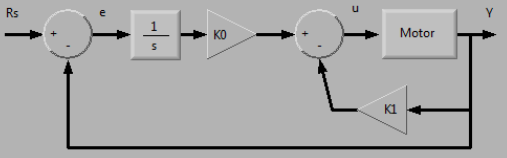
\includegraphics[scale=0.7]{img/block_diagram_angular_speed_control.png}
	\caption{Schéma blocs du système de contrôle de la
	vitesse angulaire.}
	\label{fig:block_diagram_angular_speed_control}
\end{figure}

Dans ces conditions, la fonction de transfert $T_r(s)$ est donnée
par
\begin{equation}
	T_r(s) = \frac{\frac{K_0K}{\tau}}{s^2 +\frac{K_1K+1}{\tau}s + \frac{K_0K}{\tau}}.
\end{equation}
Le système de commande en boucle fermée de la vitesse angulaire
constitue donc un système du deuxième ordre que l'on peut réexprimer
sous une forme canonique
\begin{equation}
	T_r(s) = K'\frac{\omega_n^2}{s^2 + 2\zeta\omega_n s+ \omega_n^2}
\end{equation}
où $K'$ est utilisé pour bien différencier le gain statique du système en
boucle fermée du deuxième ordre du gain statique du système en boucle
ouverte. On trouve alors
\begin{align}
	\omega_n & = \frac{K_0K}{\tau} & \zeta & = \frac{K_1K + 1}{2\sqrt{K_0K\tau}}
	& K' & = 1.
\end{align}
Pour déterminer les paramètres $K_0$ et $K_1$, on a deux spécifications
qui nous amène chacune une équation
\begin{enumerate}
	\item Un overshoot d'environ 2\%. Cette spécification a deux conséquences.
	Premièrement, elle implique que $\zeta < 1$ (sinon pas d'overshoot). Deuxièmement,
	il faut que
	\begin{equation}
		D = e^{\frac{-\pi\zeta}{\sqrt{1-\zeta^2}}} = 0.02.
	\end{equation}
	\item Un temps de réponse légèrement inférieur au temps de réponse en boucle
	ouverte (i.e. $4\tau$ pour le temps de réponse à 2\%)
	\begin{equation}
		t_R = \frac{4}{\zeta\omega_n} = \alpha \cdot 4\tau
	\end{equation}
	où $\alpha < 1$.
\end{enumerate}
Pour $\alpha = 0.9$ et avec les valeurs de $K$ et $\tau$ obtenues précedemment,
on obtient
\begin{align}
	\zeta & = 0.7797 & K_0 & = 0.6177 & K_1 & = 0.5576.
\end{align}


\section{Contrôle de la position angulaire}
Pour contrôler la position angulaire, on utilise cette fois un schéma de contrôle
avec une action intégrale, un retour d'états et un retour de sortie unitaire,
comme illustré à la figure \ref{fig:block_diagram_position_control}

\begin{figure}[ht]
	\centering
	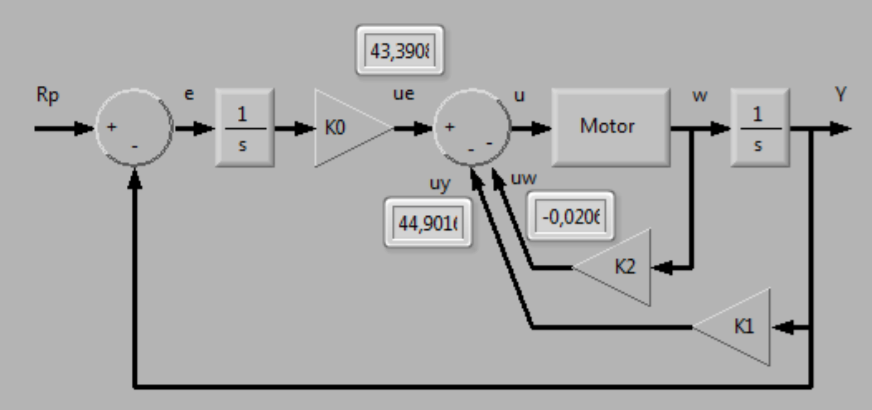
\includegraphics[width=0.8\textwidth]{img/block_diagram_position_control.png}
	\caption{Schéma blocs du système de contrôle de la position.}
	\label{fig:block_diagram_position_control}
\end{figure}

Dans ces conditions, la fonction de transfert $T_r(s)$ est donnée par
\begin{equation}
	T_r(s) = \frac{\frac{K_0K}{\tau}}{s^3 + \frac{1+K_2K}{\tau}s^2 + \frac{K_1K}{\tau}s + \frac{K_0K}{\tau}}.
\end{equation}
En plaçant judicieusement les pôles, on peut décomposer ce système en un système
du deuxième ordre dominant en série avec un système du premier ordre. Sous forme
canonique, le dénominateur peut alors s'écrire
\begin{equation}
	D(s) = (s^2 + 2\zeta\omega_ns + \omega_n^2)(s+a).
\end{equation}
On a cette fois 3 contraintes sur le systèmes
\begin{enumerate}
	\item $a \geq 10\omega_n$ pour que le pôle du système du deuxième ordre soit
	négligeable ;
	\item Le système doit avoir un overshoot $D \approx 5\%$. Cela implique que
	$\zeta < 1$ (sinon pas d'overshoot) et que
	\begin{equation}
		D = e^{\frac{-\pi\zeta}{\sqrt{1-\zeta^2}}} = 0.05.
	\end{equation}
	\item Le temps de réponse doit être de $\SI{5}{\second}$
	\begin{equation}
		t_R = \frac{4}{\zeta\omega_n} = \SI{5}{\second}.
	\end{equation}
\end{enumerate}

\end{document}